\documentclass[12pt]{article}
\usepackage[
singlelinecheck=false % The magic that stops caption centering
]{caption}
\usepackage{graphicx}
\usepackage{epstopdf}
\DeclareGraphicsRule{.tif}{png}{.png}{`convert #1 `dirname #1`/`basename #1 .tif`.png}
\usepackage{color}
\usepackage{grffile}	% makes graphicx less fussy about file names
\usepackage{longtable}
%\setlength{\LTleft}{0pt} % put longtables on the left
\usepackage{wrapfig}
\usepackage{listings}
\usepackage[toc,page]{appendix}

% Center Captions
\usepackage[justification=centering]{caption}

%% Trick to hide unused columns in tables
\usepackage{array}
\newcolumntype{H}{@{}>{\lrbox0}l<{\endlrbox}}

\usepackage{ucs}
\usepackage[english]{babel}
\usepackage{fontenc}
\usepackage{graphicx}
\usepackage{grffile}
\usepackage[hmargin=2cm,vmargin=2.5cm]{geometry}
\usepackage{fancyhdr}
\pagestyle{fancy}

%\pagestyle{headings}
\fancyfoot{}
\fancyfoot[LO,LE]{20102 \input{stamp.tex}}
\fancyfoot[RO,RE]{\thepage}

% Clickable references
\usepackage{hyperref}
\hypersetup{
    colorlinks,
    citecolor=black,
    filecolor=black,
    linkcolor=black,
    urlcolor=black
}

% Flush graphics before every new section
\usepackage{placeins}
\let\oldsection\section
\renewcommand{\section}{\FloatBarrier\oldsection} 
\let\oldsubsection\subsection
\renewcommand{\subsection}{\FloatBarrier\oldsubsection} 
\let\oldsubsubsection\subsubsection
\renewcommand{\subsubsection}{\FloatBarrier\oldsubsubsection} 

% Space out paragraphs, don't indent
\setlength{\parindent}{0.0in}
\setlength{\parskip}{0.1in}

% Macro for including schematic pages
\newcommand{\schempage}[1]{
   \begin{center}
\begin{figure}[ht!]
   \centerline{\includegraphics[width=1.3\textwidth,angle=90,keepaspectratio=true]{Figs/#1.pdf}}
    \caption{#1}
    \label{#1}
    \end{figure}
\end{center}
}


\author{
John P. Doty \and Matthew P. Wampler-Doty
}
\title{TESS Focal Plane Electronics Manual}
\date{\input{date.txt}}

\begin{document}
\begin{titlepage}
\maketitle
\begin{center}
Engineering Model Edition

\input{stamp.tex}
% \input{tag.tex}
\end{center}
\end{titlepage} 

\tableofcontents

\listoffigures

\listoftables
\pagebreak

\section{Introduction}
The TESS Focal Plane Electronics (FPE) serve as the intermediary between the four CCD sensors on a focal plane and the Data Handling Unit (DHU). Three boards make up a full FPE assembly: Video (\S \ref{Video}), Interface (\S  \ref{Interface}), and Driver (\S \ref{Driver}). The boards are connected by a 200 pin bus implemented with stacking connectors. 

Each CCD has independent clock and bias level controls. This makes the FPE robust against short-circuit failure of a CCD: in that case setting clock levels to zero will minimize fault current. Each CCD also has independent parallel clock timing to enable staggered frame store operations. This helps with the trade-off between the need to minimize the power surge due to the rapid clocking of high capacitance gates during transfer and the desire to minimize streaking by clocking as rapidly as possible. Timing of other CCD clocks is synchronous among the four CCDs.

The Driver board is not strictly necessary in a testing environment. Without the Driver board, CCD 1 and CCD 2 are fully functional. The driver board supplies clocks for CCD 3 and CCD 4. A passive jumper board that connected CCD 1 clocks to CCD 3 and CCD 2 clocks to CCD 4 would allow operation of four CCDs without a driver board, but without as much independence of clock timing and voltages.

\section{Video Board}
\label{Video}
\subsection{Input and Signal Processing Strategy}
\begin{center}
\begin{figure}[ht!]
\centerline{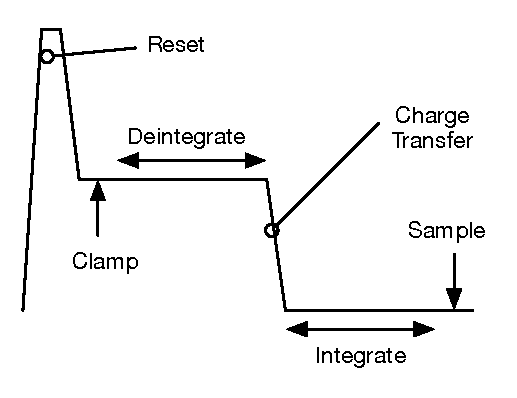
\includegraphics[keepaspectratio=true]{Figs/VideoSig/VideoSig.pdf}}
 \caption{Video Signal From CCD}
 \label{VideoSig}
 \end{figure}
\end{center}
Figure \ref{VideoSig} shows voltage versus time for a typical CCD video signal. The reset pulse resets the output node to a reference voltage that is approximately constant. However, that voltage is relatively large (10--15V) and somewhat uncertain due to switching (``kTC") noise. Then, we transfer electrons into the output node, resulting in a negative voltage step proportional to the charge.

We measure the height of the step with a three-stage process. First, we couple the signal into our measurement chains through a capacitor. On the output side of the capacitor, we have a ``clamp": a switch that forces the signal to a more reasonable level (about 3V for TESS). After we release the clamp, we ``deintegrate", averaging the baseline level before charge transfer. After charge transfer, we ``integrate", averaging the level after charge transfer. The difference in the averages is our best estimate the height of the step. We sample that difference and digitize it. In CCD jargon, this is ``correlated double sampling". Our approach combines the common ``clamp/sample" and ``Dual slope" approaches.
\subsection{Building blocks}
\subsubsection{The Video Measurement Chain}
\schempage{Chain.1}
Figure \ref{Chain.1} shows the signal path through the measurement chain.
Q2 is the active current load for the CCD output. R1 controls the current. As shown, it sinks $\approx0.8\ $mA.

U3 is the clamp. U4 buffers the clamped video. R7, R8, and C18 control the buffer gain: for maximum dynamic range we will use unity gain. U8 is the integrator that performs the signal averaging. U11 and U12 switch its inputs to control the sign of the the input signal for the deintegrate and integrate phases. 

U5 inverts the video signal, so the input to the integrator is positive during the integrate phase. It also attenuates the signal slightly to achieve greater dynamic range. R11 is reduced relative to R38 to compensate for this attenuation, keeping the correlated double sampling balanced.

U9, the ADC, uses a differential input. U6 inverts the integrator output to provide this. Filters R14/C20 and R13/C21 provide some anti-aliasing, limiting the effect of broadband noise at the outputs of U6 and U8. The ADC does not work well for a rapidly slewing input: U11 and U12 should both be off for an adequate time to allow the ADC inputs to settle before the ADC samples.

%\textcolor{red}{Jerry, Joel, and I need to get together, compare sims and reality, and define what the timing diagram should really be -jpd}

R25 feeds a current proportional to the CCD output voltage to the housekeeping circuitry for monitoring the DC component. R41 prevents the voltage on the line from exceeding the limit of the housekeeping multiplexor.

C4 should be a low hysteresis capacitor, not a common NP0. It's split because commercial capacitors of this type are difficult to obtain for values $>100\ $pF. For flight, this may be a single capacitor.

\schempage{Chain.2}
Figure \ref{Chain.2} shows the support circuitry for the measurement chain. U10 provides local voltage regulation.
\subsubsection{Drain Regulator}
\schempage{DrainRegulator}
To protect the CCD charge sense MOSFET from overvoltage, the output drain voltage range is controlled relative to the CCD reset drain.  Since the reset drain voltage controls the gate voltage on the sense MOSFET, limiting the difference to 10V limits the gate-drain voltage (see CCID80 data sheet).
\subsubsection{Per-Chip Circuitry}
\schempage{PerChip.1}
\schempage{PerChip.2}
\schempage{PerChip.3}
\schempage{PerChip.4}
\schempage{PerChip.5}
\schempage{PerChip.6}
\schempage{PerChip.7}
\schempage{PerChip.8}
Most of the Video board consists of four blocks devoted to per-chip video processing and operating bias generation. In each block, there is a video measurement chain for each segment (Figure \ref{PerChip.1}).
Figure \ref{PerChip.2} shows local fixed voltage regulation and the variable output gate regulator. Figures \ref{PerChip.3}--\ref{PerChip.6} show regulators for other variable CCD biases. Figures \ref{PerChip.7} and \ref{PerChip.8} show the DACs and housekeeping multiplexors that support these functions, as tabulated in
Table \ref{biastab} in Section \ref{param}.
\subsubsection{Charge Pumps}
\schempage{Pump}
The CCD output drains and substrate bias require modest currents at voltages outside the power supply rails. In Figure \ref{Pump}, U1, Q5, and Q6 generate a $\approx25$V peak-to-peak square wave. This is AC-coupled to a pair of Cockroft-Walton diode/capacitor ladders to make 24V (nominal) for the drain regulators, and -50V (nominal) for the substrate regulator.
\subsection{Video Board Top Level}
\schempage{Video.1}
\schempage{Video.2}
\schempage{Video.3}
\schempage{Video.4}
\schempage{Video.5}
\schempage{Video.6}
\schempage{Video.7}
\schempage{Video.8}
Figures \ref{Video.1}-\ref{Video.4} show the connections to the per-chip blocks.

Figure \ref{Video.5} shows the readout circuitry for the resistive temperature sensors on the CCD chip and camera structure. U1 is a fixed current source. U5 and U7 steer the current to the selected sensor. U6 and U8 select the resulting voltage, transmitting it to RTDCOM on the stacking connector. This goes to the housekeeping ADC on the Interface board.

Figure \ref{Video.6} shows more local voltage generation and regulation. VS12 and VS34 are regulated 4.8V for the switches in the measurement chains: these need tight regulation to control charge injection.

Figure \ref{Video.7} shows filters on the output gates. Since the output gates are next to the charge sense node, they may be a source of noise or crosstalk.

Figure \ref{Video.8} shows the control circuit for the trim heaters. Q1, Q4, and Q6 are  LM195 devices: an IC that behaves like a transistor except that it shuts down if it becomes too hot.

\subsection{Video Board Connectors}

J1, J2, J3, and J4 connect to the flexprint cables from CCD1, CCD2, CCD3, and CCD4, respectively. Table \ref{J1} shows the pinout of J1. The -1 at the end of most net names indicates that the net serves CCD1. For J2, the corresponding net names end in -2, etc. Table \ref{J5} shows the pinout for J5, which serves the external temperature sensors and heater. Table \ref{Stack} covers Js, the board stack connector.

\begin{center}
\begin{longtable}{|l|l|l|l|}
\caption{Flexprint Connector} \label{J1} \\
\hline
Connector & Pin & Net & Signal \\
\hline \endfirsthead
\caption{Flexprint Connector (continued)} \\
\hline 
Connector & Pin & Net & Signal \\
\hline
\endhead
\hline \endfoot
\input{CCD-51pin.tex}
\end{longtable}
\end{center}


\begin{table}[ht!]
\caption{Temperature Connector}
\begin{center}
\begin{tabular}{|l|l|l|l|}
\hline
Connector & Pin & Net & Comment \\
\hline
\input{TempConn.tex}
\hline
\end{tabular}
\end{center}
\label{J5}
\end{table}


\section{Interface Board}
\label{Interface}
\subsection{Building blocks}
\subsubsection{Drivers for high capacitance (parallel) clocks}
\schempage{Booster}
\schempage{ParallelPair}
\schempage{ParallelReg}
\subsubsection{Drivers for low capacitance clocks}
\schempage{SerialDriver}
\schempage{SerialRegulator}
\subsubsection{Clock drivers for one CCD}
\schempage{DriverSet.1}
\schempage{DriverSet.2}
\schempage{DriverSet.3}
\schempage{DriverSet.4}
\schempage{DriverSet.5}
\subsubsection{Power conditioning}
\schempage{ArtixPower}

Figure \ref{ArtixPower} shows the power regulators for the Artix FPGA. An RC filter on the reference insures that the 1.8V AUX power rises more slowly than the 1V core power. The 2.5V and 3.3V IO power follow the 1.8V AUX power with additional delays. This insures proper initialization. Q5 pulls down the 3.3V IO power if the 1.8V level is low, insuring that the rated maximum 2.625V difference cannot be exceeded for more than the allowed time (see Xilinx data sheet DS181). The resistors on the collectors of the pass transistors limit the surge current, and are rated to handle the fault current if the FPGA should latch up. 
\subsubsection{FPGA Reset}
\schempage{Reset}
\subsection{Interface Board Top Level}
\schempage{Interface.1}
Figure \ref{Interface.1} shows the Artix FPGA (U4). Its pin connections are too complex to draw: Table \ref{Artix} shows them. J9 is the JTAG header for FPGA debugging. J6 is the data connector to the DHU. J8 is test signals and configuration jumpers for the FPGA. Table \ref{IJ8} shows its pinout. For the pinouts of Js, the stacking connector, see Table \ref{Stack}.


\begin{table}[ht!]
\caption{FPGA Test Header}
\begin{center}
\begin{tabular}{|l|l|lH|} %Comment column hidden for now
\hline
Connector & Pin & Net & Comment \\
\hline
\input{Interface.J8.tex}
\hline
\end{tabular}
\end{center}
\label{IJ8}
\end{table}

\begin{longtable}{|Hl|l|l|} %Hide the refdes field
\caption{Artix FPGA Connections} \label{Artix} \\
\hline
Connector & Pin & Net & Signal \\
\hline \endfirsthead
\caption{Artix FPGA Connections (continued)} \\
\hline 
Connector & Pin & Net & Signal \\
\hline
\endhead
\hline \endfoot
\input{Interface.U4.tex}
\end{longtable}

\FloatBarrier
\schempage{Interface.2}
Figure \ref{Interface.2} shows support for housekeeping and temperature measurement. HKCOM is the primary housekeeping analog bus. The selected housekeeping channel will drive a current into this bus. U5 converts the current to a voltage. Full scale is $\pm27.3\,\mu$A. RTDCOM is a voltage input for the resistive temperature sensors on the CCD chips and the camera, U6 scales the voltage from the sensor circuitry on the Video board so that the full measurement range is 500\,$\Omega$ to 1500\,$\Omega$. The temperature range depends on the sensor: see Table \ref{ttab} for the nominal ranges. U3 multiplexes some voltage measurements onto HKCOM. The sense resistors are 604\,k$\Omega$. $\pm27.3\,\mu$A through 604\,k$\Omega$ is $\pm$16.5\,V, so that's full scale on these housekeeping channels.

\schempage{Interface.3}
Figure \ref{Interface.3} shows the housekeeping ADC subsystem. There are two sources of housekeeping voltage inputs to this: HKV and RTDV. Housekeeping addresses $<$112 use HKV, while the higher addresses use RTDV (see Figure \ref{Interface.2}). U1 selects which of these voltage sources to use. U6 creates a differential input for the ADC, U2.

\schempage{Interface.4}
Figure \ref{Interface.4} shows the FPGA bypass capacitors. The smallest capacitors should be closest to the power pins on the FPGA.

\schempage{Interface.5}
\schempage{Interface.6}
Figures \ref{Interface.5} and \ref{Interface.6} show the connections of the Driver Sets for CCD chips 1 and 2. The Driver Sets for CCD chips 3 and 4 are on the Driver Board.
\FloatBarrier
\schempage{Interface.7}
\FloatBarrier
Figure \ref{Interface.7} shows power input from the DHU (J7) and low voltage power conditioning. LEDs are for debugging: we will not install them on flight boards.

\section{Driver Board}
\label{Driver}
See the previous section for the DriverSet building blocks.
\schempage{Driver.1}
\schempage{Driver.2}
\schempage{Driver.3}

\section{Stack Interconnection}

\tiny{
% This is pretty crazy; here's the hack that makes this happen:
% http://tex.stackexchange.com/a/174166
    \begin{longtable}{|m{0.1\textwidth}|m{0.1\textwidth}|m{0.1\textwidth}|m{0.1\textwidth}|m{0.1\textwidth}|m{0.1\textwidth}|m{0.1\textwidth}|m{0.1\textwidth}|@{}m{0pt}@{}}
    \caption{Inter-board Stack Connections} \label{Stack} \\
    \hline
    \input{StackMap.tex}
    \end{longtable}
}

% get back to normal
\normalsize

\section{Operating Parameters and Housekeeping}
\label{param}

While the implementation details differ, the housekeeping channels and the DAC-controlled parameters share a common addressing scheme. An address is seven bits. All seven are provided to the multiplexors and their selection logic as HKA[6:0]. The most significant four bits DCS[3:0] drive the DAC selection logic: the least significant three bits are part of the serial command that sets a DAC. 

\begin{table}[ht!]
\caption{Address Map}
\begin{center}
\begin{tabular}{|l|l|l|}
\hline
Address Offset & CCD & Group \\
\hline
\input{HKmap.tex}
\hline
\end{tabular}
\end{center}
\vspace{5pt}

\label{hkmap}
\end{table}

The housekeeping ADC uses twos complement 16 bit coding. The ``Housekeeping Low'' column gives the nominal value for a code of -32768. The ``Housekeeping High'' column gives the nominal value for a code of 32767. The range is often inverted: a low code represents a high value and vice-versa.

The nominal control ranges sometimes go outside the actual range allowed for the parameters, which depend on circuit details and power supply voltages. The ``Range'' columns document the actual range in volts relative to system ground. Control is sometimes relative to another parameter. The controlling DAC chips use 12 bit unsigned coding, range 0-4095. The ``Control Low'' column gives the nominal parameter for a code of zero. The ``Control High'' column gives the nominal parameter for a code of 4095. The range is sometimes inverted: a low code represents a high value and vice-versa. If the control range is not given, the parameter is not under DAC control.
\subsection{Bias Group}
\begin{table}[ht!]
\caption{Bias Group}
\begin{center}
\begin{tabular}{|l|l|l|l|l|l|l|l|l|l|}
\hline
Address & Signal & \multicolumn{2}{c|}{Housekeeping} &  \multicolumn{2}{c|}{Control} &  \multicolumn{2}{c|}{Range} &Unit & Relative \\
Offset &  & Low & High & Low & High & Low & High &  & To  \\
\hline
\input{BiasGroup.tex}
\hline
\end{tabular}
\end{center}
\vspace{5pt}

\label{biastab}
\end{table}

\subsection{Clock Driver Group}
\begin{table}[ht!]
\caption{Clock Driver Group}
\begin{center}
\begin{tabular}{|l|l|l|l|l|l|l|l|l|l|}
\hline
Address & Signal & \multicolumn{2}{c|}{Housekeeping} &  \multicolumn{2}{c|}{Control} &  \multicolumn{2}{c|}{Range} &Unit & Relative \\
Offset &  & Low & High & Low & High & Low & High &  & To  \\

\hline
\input{ClockDriverGroup.tex}
\hline
\end{tabular}
\end{center}
\vspace{5pt}

\label{clocktab}
\end{table}
\subsection{Heater Group}
The Heater Group controls the three trim heaters on the lens barrel.
\begin{table}[ht!]
\caption{Heater Group}
\begin{center}
\begin{tabular}{|l|l|l|l|l|l|HHlH|}
\hline
Address & Signal & \multicolumn{2}{c|}{Housekeeping} &  \multicolumn{2}{c|}{Control} &  &&Unit & Relative \\
Offset &  & Low & High & Low & High & Low & High &  & To  \\
\hline
\input{HeaterGroup.tex}
\hline
\end{tabular}
\end{center}

\label{heattab}
\end{table}
\subsection{Interface Group}
\begin{table}[ht!]
\caption{Interface Group}
\begin{center}
\begin{tabular}{|l|l|l|l|HHHHlH|}
\hline
Address & Signal & \multicolumn{2}{c|}{Housekeeping} &  & &  & &Unit & Relative \\
Offset &  & Low & High & Low & High & Low & High &  & To  \\
\hline
\input{InterfaceGroup.tex}
\hline
\end{tabular}
\end{center}
\label{inttab}
\end{table}
\subsection{Thermal Group}
\begin{table}[ht!]
\caption{Thermal Group}
\begin{center}
\begin{tabular}{|l|l|l|l|HHHHlH|}
\hline
Address & Signal & \multicolumn{2}{c|}{Housekeeping} &  & &  & &Unit & Relative \\
Offset &  & Low & High & Low & High & Low & High &  & To  \\
\hline
\input{ThermalGroup}
\hline
\end{tabular}
\end{center}
\label{ttab}
\end{table}

The Thermal Group (Table \ref{ttab}) sensors are external temperature-sensitive resistors. The nominal range for the circuitry is $500\Omega$ to $1500\Omega$, which translates into the given temperature ranges. It may be useful to calibrate the board using external fixed resistors near the limits of the range.

\FloatBarrier
\begin{appendices}
\section{Acronyms and other abbreviations}
\begin{longtable}{l p{5in}}
ADC & Analog to digital converter. \\
AUX & FPGA auxiliary power. \\
CCD & Charge-coupled device. \\
DAC & Digital to analog converter. \\
HKCOM & Common output for the housekeeping multiplexors. \\
IO & Input output. \\
JTAG & Joint Test Action Group. \\
kTC & The variance of the thermal charge on a capacitor. \\
MOSFET & Metal oxide semiconductor field-effect transistor. \\
RC & Resistor-capacitor. \\
RTDCOM & Common output for the resistance temperature device multiplexors. \\


\end{longtable}

% \section{Default FPE Program}
%
% The following is the default \emph{Sequencer DSL} FPE program associated with the observatory simulator.
%
% \lstset{language=C} % Use C because it is vaguely similar
% \lstinputlisting{../Data/default_program.fpe}
%
\end{appendices}

\end{document}
